%% This is a sample manuscript marked up using the
%% AASTeX v5.x LaTeX 2e macros.

%% The first piece of markup in an AASTeX v5.x document
%% is the \documentclass command. LaTeX will ignore
%% any data that comes before this command.

%% The command below calls the preprint style
%% which will produce a one-column, single-spaced document.
%% Examples of commands for other substyles follow. Use
%% whichever is most appropriate for your purposes.
%%

%\documentclass[11pt,preprint2]{aastex}
% manuscript produces a one-column, double-spaced document:
%\documentclass[manuscript]{aastex}
%% preprint2 produces a double-column, single-spaced document:

%\documentclass{emulateapj}
\documentclass[preprint]{aastex}

\usepackage{natbib}
\usepackage{amsmath}
\bibliographystyle{apj}
\usepackage{graphicx}

\newcommand{\mintext}{\text{min}}
\newcommand{\maxtext}{\text{max}}
\newcommand{\rad}{\text{rad}}
\newcommand{\IR}{\text{IR}}
\newcommand{\ir}{\text{IR}}
\newcommand{\therm}{\text{therm}}
\newcommand{\cosmo}{\text{cosmo}}
\newcommand{\fg}{\text{fg}}
\newcommand{\res}{\text{res}}
\newcommand{\shot}{\text{shot}}
\newcommand{\SNR}{\text{SNR}}


%% Sometimes a paper's abstract is too long to fit on the
%% title page in preprint2 mode. When that is the case,
%% use the longabstract style option.

%% \documentclass[preprint2,longabstract]{aastex}

%% If you want to create your own macros, you can do so
%% using \newcommand. Your macros should appear before
%% the \begin{document} command.
%%
%% If you are submitting to a journal that translates manuscripts
%% into SGML, you need to follow certain guidelines when preparing
%% your macros. See the AASTeX v5.x Author Guide
%% for information.

%% You can insert a short comment on the title page using the command below.

%\slugcomment{Not to appear in Nonlearned J., 45.}

%% If you wish, you may supply running head information, although
%% this information may be modified by the editorial offices.
%% The left head contains a list of authors,
%% usually a maximum of three (otherwise use et al.).  The right
%% head is a modified title of up to roughly 44 characters.
%% Running heads will not print in the manuscript style.

\shorttitle{Foreground and sensitivity analysis for 21cm/Infrared studies}
\shortauthors{Neben et al.}

%% This is the end of the preamble.  Indicate the beginning of the
%% paper itself with \begin{document}.



\begin{document}

\title{3D First limits Foreground and sensitivity analysis for 21cm/Infrared intensity mapping correlation from the Epoch of Reionization}

%% Use \author, \affil, and the \and command to format
%% author and affiliation information.
%% Note that \email has replaced the old \authoremail command
%% from AASTeX v4.0. You can use \email to mark an email address
%% anywhere in the paper, not just in the front matter.
%% As in the title, use \\ to force line breaks.

\author{Abraham R. Neben\altaffilmark{1},
Brian Stalder\altaffilmark{2},
John L. Tonry\altaffilmark{2},
Jacqueline N. Hewitt\altaffilmark{1}}

\affil{\altaffilmark{1}MIT Kavli Institute, Massachusetts Institute of Technology, Cambridge, MA, 02139 USA}
\affil{\altaffilmark{2}Institute for Astronomy, University of Hawaii, 2680 Woodlawn Drive, Honolulu HI 96822}

%% Notice that each of these authors has alternate affiliations, which
%% are identified by the \altaffilmark after each name.  Specify alternate
%% affiliation information with \altaffiltext, with one command per each
%% affiliation.

%% Mark off your abstract in the ``abstract'' environment. In the manuscript
%% style, abstract will output a Received/Accepted line after the
%% title and affiliation information. No date will appear since the author
%% does not have this information. The dates will be filled in by the
%% editorial office after submission.

\begin{abstract}
aoeu
\end{abstract}

\keywords{cosmology: observations --- dark ages, reionization, first stars --- infrared: diffuse background}

\section{Introduction}

Deep radio and infrared observations are nearing detection of the first stars and galaxies from the cosmic dawn. As such sources form, they are thought to blow out ionized bubbles, eventually merging and reionizing the universe \citep{FurlanettoReview,miguelreview,PritchardLoebReview}. First generation 21\,cm observatories such the Murchison Widefield Array (MWA) \citep{tingay13,mwascience} and the Precision Array for Probing the Epoch of Reionization (PAPER) \citep{parsons14,ali15,PoberPAPER64Heating,DannyMultiRedshift} are setting ever tighter limits on redshifted neutral hydrogen emission from the neutral regions between these bubbles, and the now-underway Hydrogen Epoch of Reionization Array (HERA) \citep{deboer16} is expected to detect and characterize the EOR power spectrum in the coming years. Ultimately, the Square Kilometer Array (SKA) will image the EOR over redshift, revealing the hydrogen reionization history of the universe in detail \citep{ska}. 

At the same time, deeper galaxy redshift surveys are beginning to constrain the reionizing sources themselves. Hubble deep field observations \citep{Bouwens2011,Illingworth2013,Dunlop2013} and cluster lensing surveys are finding tens of galaxies at $6<z<10$ down to UV magnitudes of $M_{AB}\sim-17$, and extremely wide surveys are underway aiming to find rare extremely bright ones ones \citep{Schmidt2014,Trenti2011,Bradley2012}. However, current models require the contribution of far fainter galaxies down to $M_{AB}\sim-13$ \citep{Robertson2013,Alvarez2012} in order to agree with optical depth measurements \citep{planck16} from the cosmic microwave background. Deeper observations with the James Webb Space Telescope (JWST) \citep{Gardner2006} and the Wide Field Infrared Space Telescope (WFIRST) \citep{Spergel2013} will be needed to probe this crucial faint population \citep{Atek2015}.

Infrared intensity mapping offers several advantages compared to surveys. Power spectrum analyses can be sensitive to an EOR component even if the signal-to-noise in individual pixels small, and instead of being limited to the brightst galaxies, intensity mapping is sensitive to the cumulative light from \textit{all} sources. Indeed,  ionizing and Lyman-alpha radiation from EOR galaxies at $z\sim6-8$ redshifts into the near infrared, motivating intensity mapping at micron-scale wavelengths. Working around foregrounds is challenging, though. While early studies suggested angular fluctuations in infrared intensity maps traced EOR galaxies \citep[e.g.,][]{kash1,kash2,kash3}, \citet{kash4} find that given current constraints on the EOR, this is unlikely. In fact, \citet{cooray12,zemcov14} argue that intrahalo light, consisting of tidally stripped stars dispersed throughout host halos, is the best explanation for the observed fluctuation excess over known galaxy populations. This implies that even after significant foreground masking, EOR foreground emission in wide field infrared surveys is of order $10^4$ times brighter than EOR emission at $\sim10'$ scales.

Given these bright foregrounds, cross correlation with 21\,cm maps may in fact be the \textit{only} way to extract the diffuse EOR component of the near infrared background. The synergy is clear: the galaxies sourcing reionization generate strong Ly-$\alpha$ emission, while the neutral regions between them glow at rest frame 21\,cm. On scales larger than typical ionized bubbles, bright spots in IR maps likely correspond to ionized regions, and thus, 21\,cm dark spots, and vice versa, sourcing an anticorrelation seen in EOR simulations by \citet{StarsAndReionization,silva12,mao14,heneka16}. 

A similar anticorrelation on large scales is found by \citet{lidz09,park14} in simulations of 21\,cm cross correlation with galaxy surveys, but conducting redshift surveys both wide and deep enough to cross correlate with 21\,cm maps is an  challenge due to the wildly different spatial scales probed by 21\,cm experiments and deep galaxy surveys. The Hubble Ultra Deep Field, for instance, could fit inside a single resolution element in an MWA map. It may be possible to cross-check the ionization environment of deep JWST sources by comparing the brightness temperature in the 21\,cm map \citep{beardsley15}, but even after order $\sim100$\,hour integrations such detections will be near JWST limiting sensitivities \citet{zackrisson11}.

In contrast, intensity allows similar science with shallower observations, though imperfect radio and infrared foreground subtraction will leak largely uncorrelated power into the cross correlation analysis which must be averaged out over large fields of view. Fortunately the planned Transiting Exoplanet Survey Satellite \citep{ricker14} and the proposed SPHEREx mission \citep{ScienceWithSpherex,SpherexWhitePaper} would collect all sky near infrared maps, and many ground-based near infrared surveys with few degree fields such as the Dark Energy Survey \citep{des16}, Pan-STARRS \citep{tonry12}, and the Asteroid Terrestrial-impact Last Alert System (ATLAS) \citep{tonry11} are coming online. In the low frequency radio, the MWA has performed a deep survey of 400 square degrees at high galactic latitude \citep{beardsley16}, and HERA will survey $\sim2000$ square degrees along a zenith strip \citep{dillonmapmaking}. 

With wide and deep IR and low frequency radio surveys happening now and on the horizon, we study in this paper the real world prospects of detecting the cross correlation of diffuse 21cm and Ly-alpha emission from the EOR. We begin in Section 1 with a cross correlation analysis of radio and near infrared catalogs, setting upper limits on the level of foreground correlation, the presence of which would mask the cosmological correlation in sufficiently deep images. We then assess the correlation of faint, unresolved emission through a prototype 21cm/IR correlation analysis between wide band MWA and ATLAS images over a 10 degree field of view. After foreground subtraction and masking, we estimate typical foreground residual levels, and synthesize these with noise predictions into a sensitivity analysis for a larger scale image cross correlation experiment. We also make sensitivity predictions for a cube cross correlation experiment, quantifying the required infrared spectral resolution and taking advantage of avoidance of radio foregrounds using the ``EOR window''.

\section{Power spectrum and correlation conventions}
\label{sec:pspecconventions}

\subsection{Power spectrum definitions}

We define the 3D power spectrum $P(\vec{k})$ of the image cube $I(x,y,z)$ following \citet{ewallwice14} as 
\begin{equation}
	P(\vec{k}) = \frac{\langle|\tilde{I}(\vec{k})|^2\rangle}{V}
\end{equation}
where
\begin{equation}
	\tilde{I}(\vec{k})=dV\sum_{\vec{x}}I(\vec{x})e^{i\vec{k}\cdot\vec{x}}
\end{equation}
and $V$ is the survey volume, and $dV$ is the voxel size.

Similarly, over narrow fields of view, the angular power spectrum $C_\ell$ of a 2D (e.g, broad band) image $I(\vec{\theta})$ can be shown to be approximately
\begin{equation}
\label{eqn:Cldef0}
	C(\vec{\ell}) = \frac{\langle|\tilde{I}(\vec{\ell})|^2\rangle}{\Omega} 
\end{equation}
where
\begin{equation}
	\tilde{I}(\vec{\ell})=d\Omega\sum_{\vec{\theta}}I(\vec{\theta})e^{i\vec{\ell}\cdot\vec{\theta}}
\end{equation}
and $\Omega$ is the survey solid angle, and $d\Omega$ is the pixel size. Thus, we need only evaluate a fourier transform to estimate $C_\ell$ over a narrow field of view. Writing this out in detail, we find\footnote{IS IT REALLY RIGHT THAT ALL THESE PEOPLE WROTE IT UP WRONG? ARE THERE DIFFERENT NORMALIZATIONS OF C$\ell$ ? Note that the normalization of $d\theta^2/N^2$ has been misstated as $1/N^2$ by \citet{zemcov14} (Eqn. 3 of their supplement), $d\theta$ by \citet{cooray12} (Eqn. 1 of their supplement), and $N^2d\ell^2/(2\pi)^2$ by \citet{thacker15} (Eqn. B3). Using Eqn. \ref{eqn:elldef}, the last form can be shown equal $1/d\theta^2$.} 
\begin{equation}
\label{eqn:Cldef}
	C(\ell(a,b))=\left\langle\left|\sum_{m,n}I(m,n)\exp\left(-\frac{2\pi i}{N}  (am+bn)\right)\right|^2\right\rangle\frac{d\theta^2}{N^2}
\end{equation}
where $d\theta=d\theta_x=d\theta_y$ is the pixel size, $N\equiv N_x=N_y$ is number of pixels on a side of a square image, and $\ell=\sqrt{\ell_x^2+\ell_y^2}$, where 
\begin{eqnarray}
\ell_x&=&2\pi a/N d\theta \label{eqn:elldef}\\
\ell_y&=&2\pi b/Nd\theta \label{eqn:elldef2}
\end{eqnarray}

Note that $C_\ell$ has the units of $[I^2d\theta^2]$. We will generally work with the dimensionally more intuitive power spectrum $\Delta(\ell)$, given by
\begin{equation}
	\Delta(\ell)=\sqrt{\frac{\ell^2}{2\pi}C(\ell)}
\end{equation}
which has the same units as I because $\ell$ has units of 1/rad. 

The 3D power spectrum is often cylindrically binned to $(k_\perp,k_\parallel)$ space where $k_\perp^2\equiv k_x^2+k_y^2$ represents modes perpendicular to the line of sight, and $k_\parallel=k_z$ represents modes along the line of sight. We show in Appendix \ref{sec:pspecrelation}  that this cylindrically binned power spectrum is related to the angular power spectrum of a broad band image (over a narrow field of view) as
\begin{equation}
P(k_\perp,k_\parallel=0)=D_c^2 \Delta D_c C_{\ell(k_\perp)}	
\end{equation}
with $\ell=D_c k_\perp$, where $D_c$ is the comoving line of sight distance to the center of the cube, and $\Delta D_c$ is the comoving depth of the cube.

\subsection{Cross spectrum vs. coherence}

We extend the definition of the angular power spectrum given in Eqn. \ref{eqn:Cldef0} to the cross spectrum as
\begin{equation}
\label{eqn:Cldefcross}
	C_{A,B}(\vec{\ell}) = \frac{\langle \tilde{I}_A^*(\vec{\ell})\tilde{I}_B(\vec{\ell})\rangle}{\Omega}
\end{equation}
where $A$ and $B$ denote the 21\,cm and the IR fields. The cross spectrum is a quantity which ranges between $\pm(C_{A}(\vec{\ell})C_{B}(\vec{\ell}))^{1/2}$ depending on how correlated or anti-correlated the two fields are. 

The cross spectrum is thus often renormalized as  
\begin{equation}
\label{eqn:Cldefcross}
	c_{A,B}(\vec{\ell}) \equiv \frac{C_{A,B}(\vec{\ell}) }{\sqrt{C_A(\vec{\ell})  C_B(\vec{\ell}) }}
\end{equation}
where $c$ is known as the coherence. The coherence quantifies the fractional correlation of the two fields, and is insensitive to a simple rescaling of either one. However, large foreground residuals afflicting either field will substantially bias the coherence towards zero \citep{lidz09,furlanettolidz07}. 


\section{3D intensity mapping}

NEED TO START REJIGGERING THIS SECTION

\subsection{Sensitivity framework}
We adapt the cross spectrum sensitivity results of \citet{lidz09} to our case of measuring the 21\,cm--IR cross spectrum of broadband images with noise and foreground residuals. 
\begin{equation}
\label{eqn:sense1}
	\sigma_{21,\IR}^2(\vec{\ell})=\frac{1}{2}[C^2_{21,\IR}(\vec{\ell})+\sigma_{21}(\vec{\ell})\sigma_{\IR}(\vec{\ell})]
\end{equation}
\begin{equation}
\label{eqn:sense2}
	\sigma_{21}^2(\vec{\ell})=[C_{21,\cosmo}(\vec{\ell})+C_{21,\fg}(\vec{\ell})+C_{21,\therm}(\vec{\ell})]^2
\end{equation}

\begin{equation}
\label{eqn:sense3}
	\sigma_{\IR}^2(\vec{\ell})=[C_{\IR,\cosmo}(\vec{\ell})+C_{\IR,\fg}(\vec{\ell})+C_{\IR,\shot}(\vec{\ell})]^2
\end{equation}
where $\cosmo$ signifies the cosmological component of the signal from the EOR, $\fg$ signifies residual foregrounds, $\therm$ signifies thermal noise in 21\,cm images, and $\shot$ signifies photon shot noise in IR images. 

\subsection{Broad band correlation experiment sensitivity}

Though these are the general forms of these equations, we omit the thermal and photon shot noise contributions in the rest of this section, as we have shown them to be negligible in Sections \ref{sec:pspec21fg} and \ref{sec:pspecIRfg}. We also omit the sample variance terms as they become important only in the SNR $\sim1$ regime. 

Now suppose we evaluate the 2D cross spectrum as in Eqn. \ref{eqn:Cldefcross}, and bin it in annuli such that bin $\ell$ contains containing $N_\ell$ $\ell$ cells. Then the noise decreases as
\begin{equation}
	\sigma_{21,\IR}^2(\ell) = \frac{\sigma_{21,\IR}^2(\vec{\ell}) }{N_\ell}
\end{equation}

Then substituting Eqns. \ref{eqn:sense1}-\ref{eqn:sense3} into the above equation and omitting factors of order unity, we find that the signal to noise ratio $\SNR(\ell)$ of the measurement of cross spectrum mode $\ell$ is given by
\begin{equation}
	\SNR(\ell) = \sqrt{
		2N_\ell
	\left(\frac{C_{21,\cosmo}(\vec{\ell})  }{ C_{21,\fg}(\vec{\ell}) }\right)
	\left(\frac{C_{\IR,\cosmo}(\vec{\ell})  }{ C_{\IR,\fg}(\vec{\ell}) }\right)
	}
\end{equation}

Let us optimize the SNR by using only two bins, $\ell_1=\ell_\text{max}/4$ and $\ell_2=3\ell_\text{max}/4$, where $\ell_\text{max}=\pi/d\theta$ and the cell size is given by $d\ell=2\ell_\text{max}/N=2\pi/\theta_\text{FOV}$. Now let's derive some intuition into $N_\ell$ by writing it as $N_\ell=(\ell_\text{max}/d\ell)^2F_\ell=(\theta_\text{FOV}/2d\theta)^2F_\ell$, where $F_\ell$ is an order unity quantity equal to the fraction of all $\vec{\ell}$ cells included in bin $\ell$.

%\begin{equation}
%	\SNR(\ell) = \frac{\theta_\text{FOV}}{2d\theta}  \sqrt{2F_\ell
%	\left(\frac{C_{21,\cosmo}(\vec{\ell})  }{ C_{21,\fg}(\vec{\ell}) }\right)
%	\left(\frac{C_{\IR,\cosmo}(\vec{\ell})  }{ C_{\IR,\fg}(\vec{\ell}) }\right)
%	}
%\end{equation}

\begin{eqnarray}
	\SNR(\ell)&=&XX \left(\frac{\theta_\text{FOV}}{20^\circ}\right)\left(\frac{5'}{d\theta}\right)\left(\frac{F_\ell}{1}\right)^{1/2}\left(\frac{\alpha_{21}}{0.1}\right)^{1/2}
\end{eqnarray}
where the fraction of 21\,cm foregrounds remaining after subtraction is given by $\alpha_{21}\equiv C_{21,\res}/C_{21,\fg}$, and the fraction of IR foregrounds removed by masking is assumed to be XXX. REMEMBER, WE CAN'T MASK OUR WAY TO THE SIGNAL BECAUSE OF THE INTRAHALO
-LIGHT


\subsection{3D correlation experiment sensitivity}

\begin{figure*}[h]
\centering
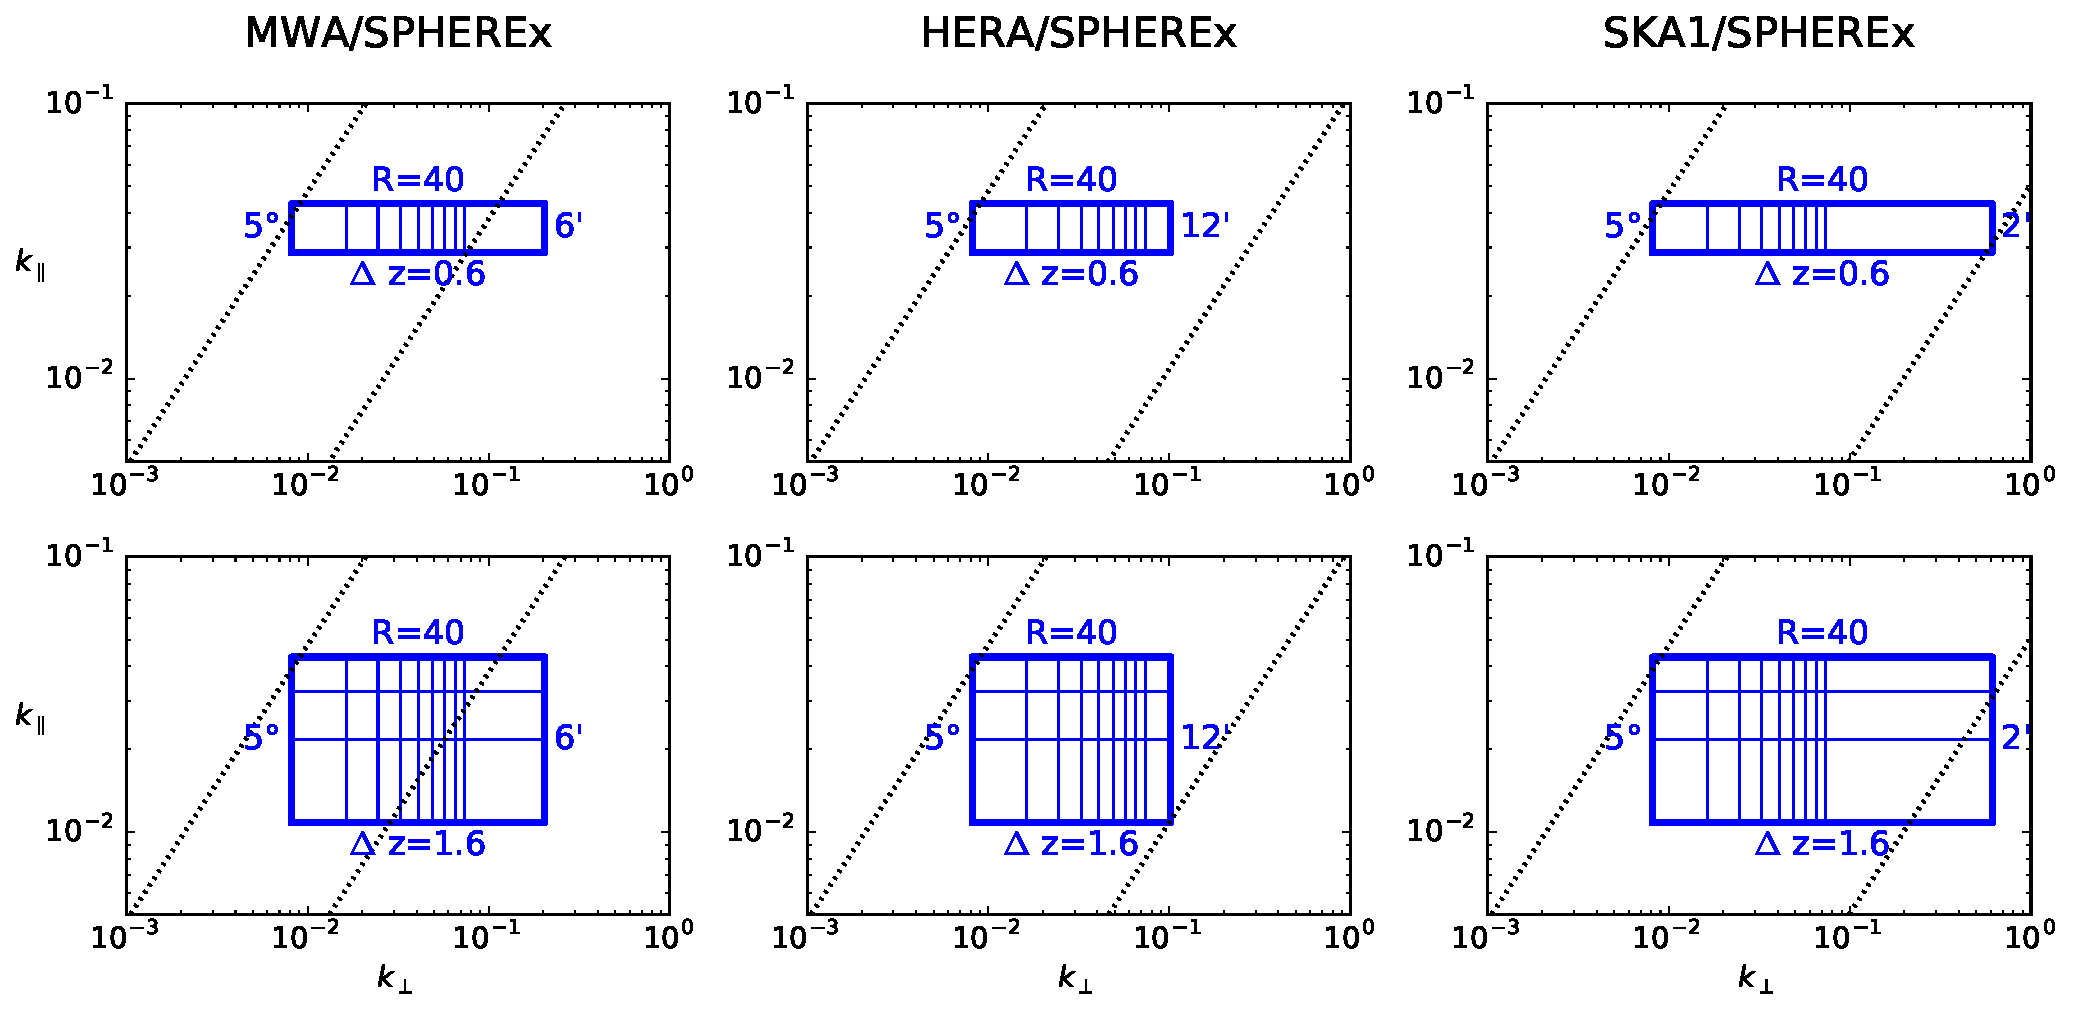
\includegraphics[width=6.5in]{images/kspace_overlap.pdf}
\caption{aoeuaoeuaoeu}
\label{fig:corgrid}
\end{figure*}

\begin{figure*}[h]
\centering
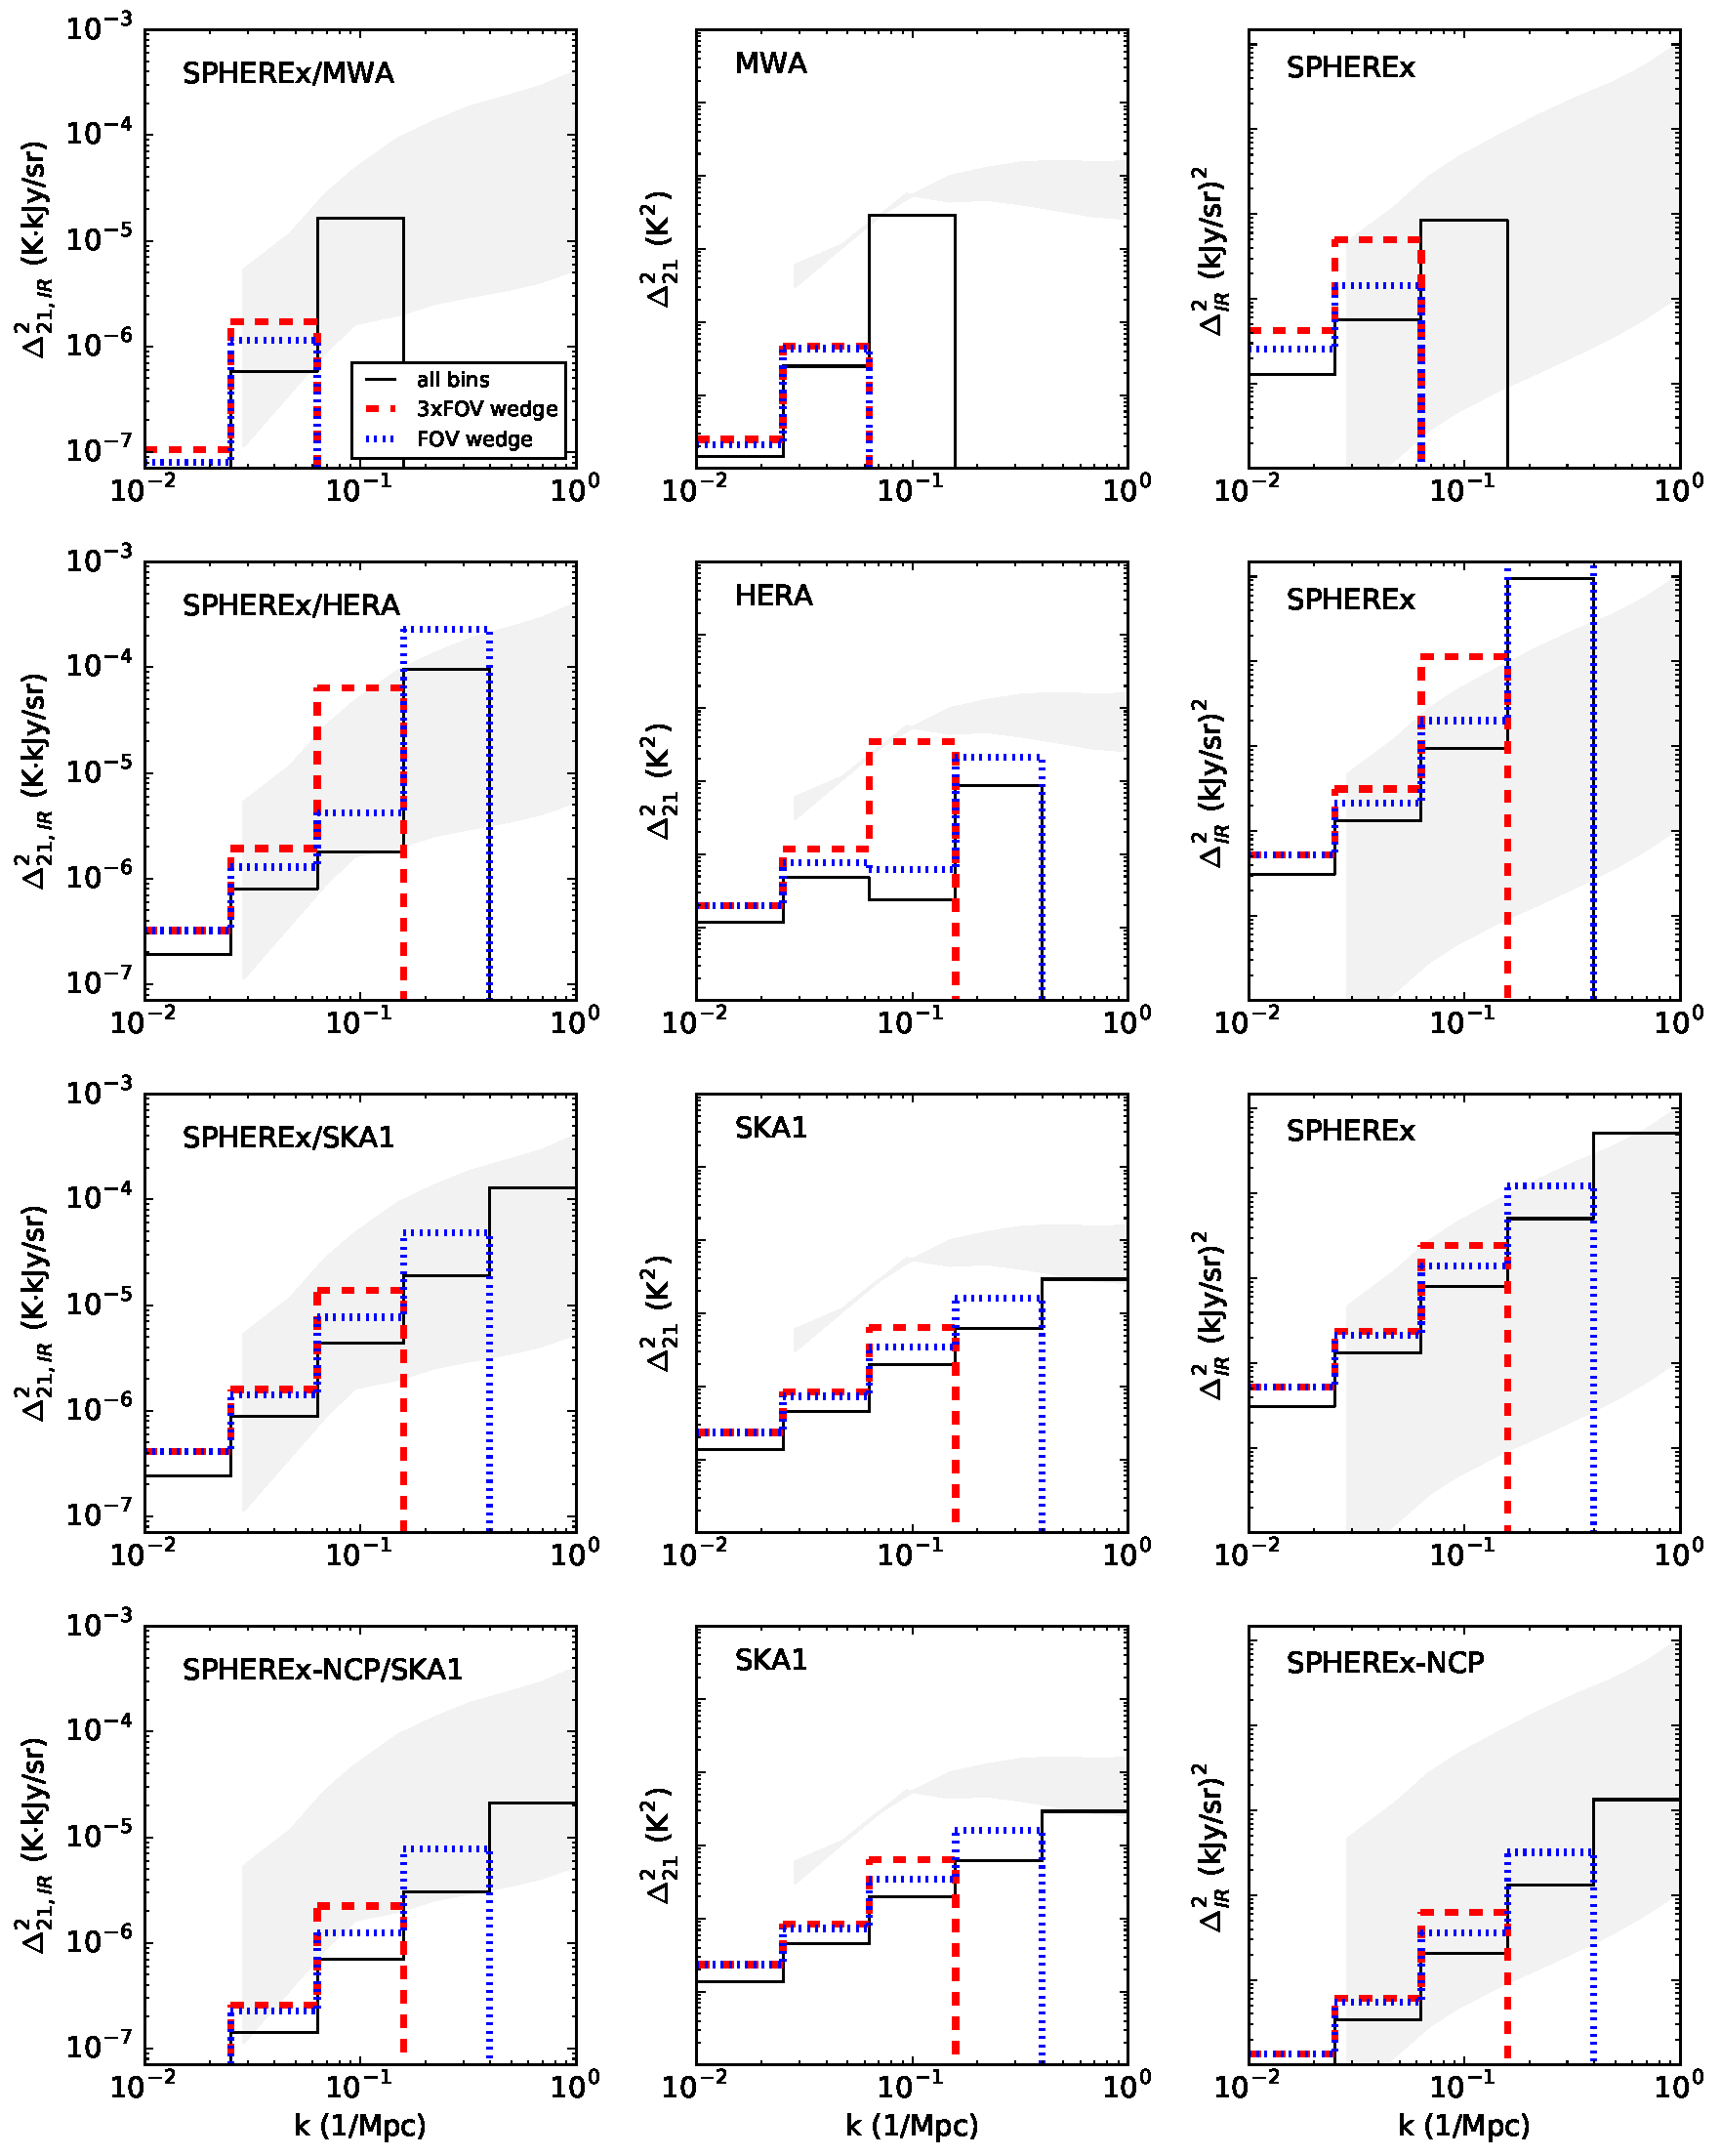
\includegraphics[width=7in]{images/cross_and_auto_sensitivity_for_diff_expts.pdf}
\caption{aoeuaoeuaoeu}
\label{fig:corgrid}
\end{figure*}






\section{Discussion}

\appendix

\section{Power spectrum of photon shot noise}
\label{sec:Pshot}

In Sec. \ref{sec:pspecIRfg} we measure the maximum airglow to be $I_\text{air}=5\times10^3$ kJy/sr, and in this appendix we calculate the power spectrum of this photon shot noise. We must observe that the mean number of photons collected by a pixel during each observation is $\langle N_\text{ph}\rangle=I_\text{air}At_\text{int} \Delta f d\theta^2/hf$, where $A=(0.5\,\text{m})^2$ is the collecting area of ATLAS, $t_\text{int}=30\,$sec, $\Delta f$ and $f$ are the frequency bandwidth and center frequency of I band, and $d\theta$ is the pixel size. The passband has $\Delta\lambda=150\,$nm and $\lambda=800\,$nm. 

The shot noise contribution to the power spectrum is given by
\begin{equation}
C_{\IR, \shot}(\vec{\ell}) = \left\langle\left|\sum_{m,n}I_\shot(m,n)e^{-2\pi i(ma+nb)/N}\right|^2\right\rangle \frac{d\theta^2}{N^2}
\end{equation}
where $I_\shot(m,n)\equiv I(m,n)-\langle I(m,n)\rangle$ denotes the photon shot noise contribution to pixel (m,n), and $N$ is the number of pixels on each side of the square image. Then using the fact that the shot noise is uncorrelated between different pixels, we find
\begin{equation}
C_{\IR, \shot}(\vec{\ell}) = \sum_{m,n}\langle I^2_\shot(m,n)\rangle \frac{d\theta^2}{N^2}
\end{equation}
Note that $I(m,n)=N_\text{ph}(m,n)hf/\Delta f A t_\text{int}d\theta^2$ and $\langle N_\text{ph}^2\rangle = \langle N_\text{ph}\rangle$, so we have
\begin{equation}
C_{\IR, \shot}(\vec{\ell}) = \langle N_\text{ph}\rangle \left(\frac{hf}{\Delta f A t_\text{int}d\theta^2}\right)^2 d\theta^2
\end{equation}

\begin{equation}
C_{\IR, \shot}(\vec{\ell}) =\frac{I_\text{air}h\lambda}{\Delta \lambda A t_\text{int}}
\end{equation}

NOTE THAT $C_\shot$ DECREASES WITH BINNING IN THE CROSS SPECTRUM, BUT NOT IN THE AUTO SPECTRUM!!!!!!!!!!!!!!!!!!!!!!!

\section{Relation between the power spectrum of image cubes and broadband images}
\label{sec:pspecrelation}

NOTE THAT THIS ONLY HOLDS FOR LARGE ELL OVER A SMALL FIELD OF VIEW

We focus in this paper on the spherical power spectrum of broadband images, $C_\ell$,  instead of that of image cubes, $P(\vec{k})$, as 21\,cm observations have focused on. Here we work out the relation between the two to facilitate comparison with past 21\,cm power spectrum results. In particular, we calculate the scaling factor $B$ relating the purely transverse modes of the power spectrum $P(k_\perp,k_\parallel=0)$ of a image cube $I(\theta_x,\theta_y,f)$ to the spherical power spectrum of a broad band image $C_\ell$ as
\begin{equation}
P(k_\perp,k_\parallel=0) = B C_{\ell(k_\perp)}
\end{equation}

Using the fourier transform convention discussed in Sec. \ref{sec:pspecconventions}, the left side of the equation is given by
\begin{equation}
P(k_\perp,k_\parallel=0) = \frac{1}{N_\perp^2 N_\parallel dV}\langle|\tilde{I}(k_x,k_y,k_\parallel=0)|^2\rangle
\end{equation}
where $N_\perp\equiv N_x=N_y$ is the number of pixels in each of the two transverse dimensions of the image cube, and $N_\parallel$ is the number of pixels in the line of sight (ie, frequency) dimension. The comoving pixel volume is $dV = (D_c d\theta)^2 (\Delta D_c/N_\parallel)$, where $D_c$ is the line of sight comoving distance from the present day to the center of the cube, and $\Delta D_c$ is the comoving line of sight thickness of the cube. Lastly, recall that $k_\perp$ is related to $k_x$ and $k_y$ as $k_\perp=\sqrt{k_x^2+k_y^2}$.

Now substituting the definition of the fourier transform, we find

\begin{equation}
P(k_\perp,k_\parallel=0) =\frac{1}{N_\perp^2 N_\parallel dV}\left\langle\left|dV\sum_{\theta_x,\theta_y,f}I(\theta_x,\theta_y,f)e^{iD_c(k_x\theta_x+k_y\theta_y)}\right|^2\right\rangle
\end{equation}

Simplifying and writing this in terms of the broadband image $I_{\Delta f}(\theta_x,\theta_y)\equiv\frac{1}{N_\parallel}\sum_f  I(\theta_x,\theta_y,f)$, we find

\begin{equation}
P(k_\perp,k_\parallel=0) =(D_c^2 \Delta D_c)
\frac{d\theta^2}{N_\perp^2}\left\langle\left|\sum_{\theta_x,\theta_y}I_{\Delta f}(\theta_x,\theta_y)e^{iD_c(k_x\theta_x+k_y\theta_y)}\right|^2\right\rangle
\end{equation}

Now denote $k_x=a\cdot dk$, $k_y=b\cdot dk$, $\theta_x=m\cdot d\theta$, and $\theta_y=n\cdot d\theta$, where $dk = 1/N_\perp D_c d\theta$. 

\begin{equation}
P(k_\perp(\ell(a,b)),k_\parallel=0) =(D_c^2 \Delta D_c)
\frac{d\theta^2}{N_\perp^2}\left\langle\left|\sum_{m,n}I_{\Delta f}(m,n)e^{2\pi i(am + bn)/N_\perp}\right|^2\right\rangle
\end{equation}

Comparing with Equations \ref{eqn:Cldef}, \ref{eqn:elldef}, and \ref{eqn:elldef2}, we see that $B\equiv P(k_\perp,k_\parallel=0)/ C_{\ell(k_\perp)}=D_c^2 \Delta D_c$ and $\ell=D_c k_\perp$.

%% The reference list follows the main body and any appendices.
%% Use LaTeX's thebibliography environment to mark up your reference list.
%% Note \begin{thebibliography} is followed by an empty set of
%% curly braces.  If you forget this, LaTeX will generate the error
%% "Perhaps a missing \item?".
%%
%% thebibliography produces citations in the text using \bibitem-\cite
%% cross-referencing. Each reference is preceded by a
%% \bibitem command that defines in curly braces the KEY that corresponds
%% to the KEY in the \cite commands (see the first section above).
%% Make sure that you provide a unique KEY for every \bibitem or else the
%% paper will not LaTeX. The square brackets should contain
%% the citation text that LaTeX will insert in
%% place of the \cite commands.

%% We have used macros to produce journal name abbreviations.
%% AASTeX provides a number of these for the more frequently-cited journals.
%% See the Author Guide for a list of them.

%% Note that the style of the \bibitem labels (in []) is slightly
%% different from previous examples.  The natbib system solves a host
%% of citation expression problems, but it is necessary to clearly
%% delimit the year from the author name used in the citation.
%% See the natbib documentation for more details and options.

\bibliography{xcor_paper3D}


\end{document}
